\section{II. Luật chơi Saboteur}

% 1
\begin{frame}
\frametitle{Bộ bài Saboteur đầy đủ}

\begin{figure}[H]
    \centering
    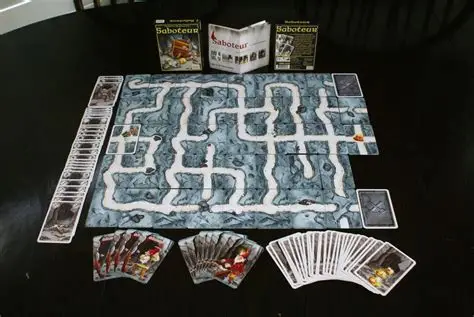
\includegraphics[width=0.6\linewidth]{luat_choi/image.png}
\end{figure}

\end{frame}

% 2
\begin{frame}
\frametitle{Tổng quan Saboteur}
\begin{columns}
    \column{0.5\textwidth}
    \textbf{Tổng quan và mục tiêu}
    \begin{itemize}
        \item Số người chơi: 3--10.
        \item Mục tiêu:
        \begin{itemize}
            \item \textbf{Gold-Diggers}: mở đường từ Start đến Goal chứa vàng.
            \item \textbf{Saboteurs}: phá để Gold-Diggers không thể đến được vàng.
        \end{itemize}
    \end{itemize}

    \column{0.5\textwidth}
    \textbf{Trang bị trong bộ Saboteur}
    \begin{itemize}
        \item 40 Thẻ đường (path cards): gồm 31 thẻ thông, 9 thẻ cụt
        \item 27 Thẻ hành động (action cards)
        \item 11 Thẻ vai trò (role cards)
    \end{itemize}
\end{columns}

\end{frame}

% 3
\begin{frame}
\frametitle{Hình minh họa bộ thẻ và bàn chơi}

\begin{figure}[H]
    \centering
    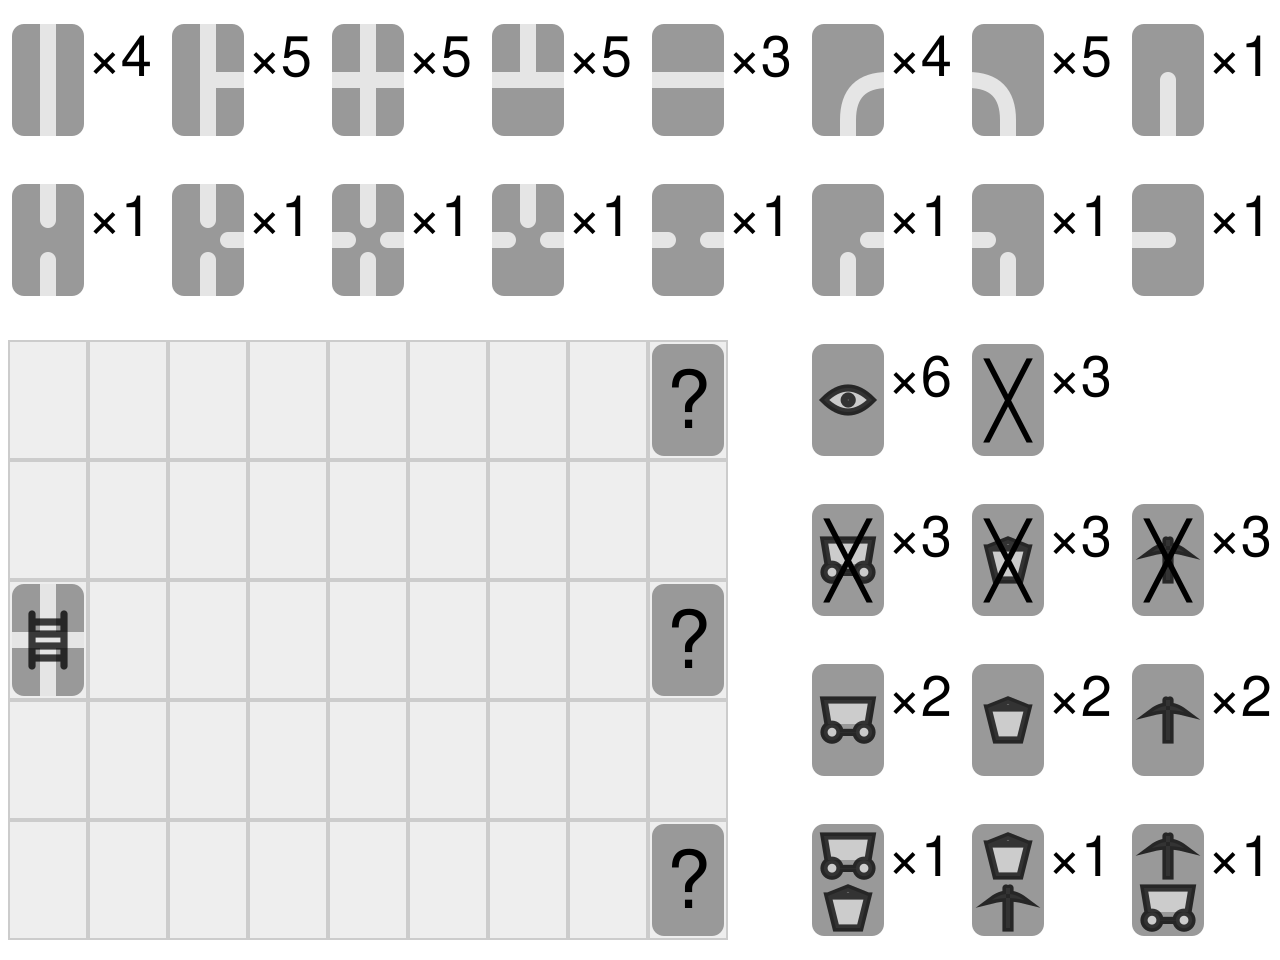
\includegraphics[width=0.6\linewidth]{luat_choi/saboteurCards.png}
    \label{fig:cards-and-board}
\end{figure}

\end{frame}

% 4
\begin{frame}
\frametitle{Bố trí bàn chơi (Setup)}
\begin{itemize}
    \item Đặt thẻ Start ở giữa bên trái.
    \item Đặt 3 thẻ Goal úp cách Start 7 khoảng thẻ: 1 giữa, 1 trên, 1 dưới.
    \item Vai trò và số thẻ phát cho mỗi người
    \item Tất cả những lá bài còn lại được xáo lại thành chồng và để úp xuống bàn.
\end{itemize}
\begin{columns}
    \column{0.5\textwidth}
    \textbf{Số lượng vai trò}
    \begin{table}[h]
    \centering
        \begin{tabular}{|c|c|c|c|c|c|c|}
        \hline
        Tổng số Người chơi & 3 & 4 & 5 & 6 & 7 & 8  \\ \hline
        Số Saboteurs     & 1 & 1 & 2 & 2 & 3 & 3 \\ \hline
        Số Gold-Diggers  & 2 & 3 & 3 & 4 & 3 & 4  \\ \hline
        \end{tabular}
        \label{tab:total-roles}
    \end{table}

    \column{0.5\textwidth}
    \textbf{Số thẻ phát cho mỗi người}
    \begin{table}[h]
    \centering
        \begin{tabular}{|c|c|c|c|c|c|c|}
        \hline
        Tổng số Người chơi      & 3 & 4 & 5 & 6 & 7 & 8 \\ \hline
        Thẻ mỗi người      & 6 & 6 & 6 & 5 & 5 & 4 \\ \hline
        \end{tabular}
        \label{tab:cards-per-player}
    \end{table}
\end{columns}

\end{frame}


% 5
\begin{frame}
\frametitle{Luật chơi Saboteur}

    \begin{itemize}
    \item Lượt xoay chiều kim đồng hồ.
    \item Mỗi lượt chọn một trong các hành động:
    \begin{enumerate}
        \item Đặt thẻ đường (path card).
        \item Chơi thẻ hành động (action card).
        \item Bỏ thẻ (discard).
    \end{enumerate}
    \item Sau khi xong lượt của mình, người chơi bốc lên thẻ trên cùng của deck, lượt chơi tiếp tục qua người tiếp theo.
    \item Gold-Diggers thắng khi có đường nối (phải là đường thông) từ start tới goal chứa vàng. Saboteurs thắng khi tất cả đã hết bài mà vẫn chưa nối được đường tới vàng.
    \end{itemize}

\end{frame}

% 6
\begin{frame}
\frametitle{Thẻ đường (Path Cards)}

    \begin{figure}[H]
        \centering
        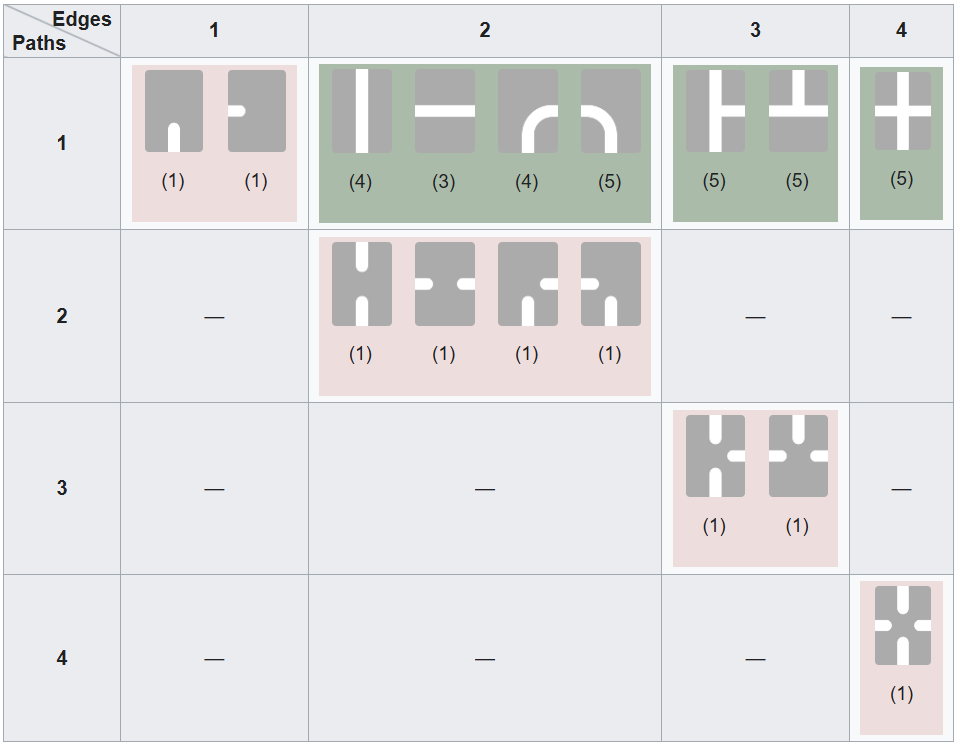
\includegraphics[width=0.5\linewidth]{luat_choi/pathCards.png}
    \end{figure}

\end{frame}

% 7
\begin{frame}
\frametitle{Thẻ đường (Path Cards)}

\begin{columns}
    \column{0.5\textwidth}
    \textbf{Phân loại thẻ Đường}  \\
    \begin{itemize}
        \item \textbf{Thẻ đường thẳng}: nối liền hai đầu theo trục ngang hoặc dọc.
        \item \textbf{Thẻ giao nhau}: có nhiều nhánh rẽ, cho phép mở rộng đường theo nhiều hướng.
        \item \textbf{Thẻ cụt (dead-end)}: Có thể nối với các thể khác nhưng không được tính là thông đường.
        \item Các cạnh thẻ không có lối được tính là tường,  khiến người chơi không thể nối đường theo hướng đó.
    \end{itemize}
    

    \column{0.5\textwidth}
    \textbf{Cách đặt thẻ Đường hợp lệ}  \\
    Một thẻ Đường được xem là hợp lệ khi thỏa các điều kiện sau:
    \begin{itemize}
        \item Các đầu đường (lối ra) trên thẻ mới phải khớp với đầu đường của thẻ đã có trên bàn: đường nối với đường, tường nối với tường.
        \item Không được tạo ra một kết nối trái ngược (ví dụ: đầu đường mở nối vào tường bịt).
        \item Thẻ phải được đặt kề cạnh một thẻ đã có sẵn trong mạng lưới (không được “nhảy cóc”).
        % \item Người chơi không được phá vòng lặp đang tồn tại trừ khi dùng thẻ hành động chuyên biệt.
    \end{itemize}

\end{columns}
\end{frame}

% 8
\begin{frame}
\frametitle{Thẻ đường (Path Cards)}

\begin{columns}
    \column{0.5\textwidth}
    \textbf{Quy tắc xoay thẻ}  \\
    Tất cả thẻ Đường đều có thể được xoay 180° trước khi đặt xuống.  
    \begin{itemize}
        \item Người chơi không được xoay 90°; chỉ xoay 180° vì cấu trúc hầm được thiết kế theo hai hướng chính.
        \item Sau khi xoay, thẻ vẫn phải thỏa điều kiện kết nối hợp lệ như đã nêu ở mục trên.
    \end{itemize}


    \column{0.5\textwidth}

    \textbf{Phá đường bằng thẻ Bomb}  \\
    Thẻ \emph{Bomb} là thẻ hành động dùng để phá hủy một thẻ Đường đã được đặt trên bàn.
    \begin{itemize}
        \item Người chơi chọn một thẻ Đường bất kỳ (trừ thẻ Start và thẻ Goal) để loại bỏ.
        \item Sau khi phá, ô trống được để lại và không có thẻ nào tự động dịch chuyển vào.
        \item Bomb không được dùng để phá thẻ trên tay người chơi, chỉ phá thẻ đã đặt.
    \end{itemize}
\end{columns}
\end{frame}


% 9
\begin{frame}
\frametitle{Thẻ hành động (Action Cards)}

\begin{columns}
    \column{0.5\textwidth}
    
    Các thẻ hành động ảnh hưởng trực tiếp đến khả năng đặt thẻ đường hoặc quan sát thông tin trong ván chơi.  
    Trong game có \textbf{3 loại công cụ}: 
    \begin{itemize}
        \item Xe đẩy (\textit{Cart})
        \item Xẻng (\textit{Shovel})
        \item Mũ (\textit{Hat})
    \end{itemize}

    \column{0.5\textwidth}
    Nếu người chơi bị phá \textbf{bất kỳ một trong ba công cụ}, họ \textbf{không thể đặt thẻ đường}.  
    Để sửa, người chơi phải dùng thẻ Repair tương ứng.

    \begin{itemize}
        \item \textbf{Repair đơn}: sửa đúng 1 công cụ được chỉ định trên thẻ.
        \item \textbf{Repair kép}: sửa 1 trong 2 công cụ hiển thị trên thẻ (Có biến thể có thể sửa cả hai đồng thời).
    \end{itemize}
\end{columns}
\end{frame}

% 10
\begin{frame}
\frametitle{Thẻ hành động (Action Cards)}

    \begin{table}[H]
    \centering
    \begin{tabular}{|c|p{7cm}|c|}
    \hline
    \textbf{Loại thẻ} & \textbf{Công dụng} & \textbf{Số lượng} \\ \hline
    Sabotage & Phá 1 công cụ: Cart, Shovel hoặc Hat. Người bị phá không thể đặt Path cho đến khi được sửa. & 9 \\ \hline
    Repair   & Sửa công cụ bị phá. Gồm: 6 thẻ đơn (mỗi loại công cụ 2 thẻ), 3 thẻ kép. & 9 \\ \hline
    Map      & Cho phép xem lén 1 trong 3 thẻ Goal. Không được tiết lộ thông tin trừ khi tự nguyện. & 6 \\ \hline
    Bomb & Phá hủy 1 Path card trên bàn (trừ Start và 3 Goal). Thẻ bị phá được loại khỏi mỏ. & 3 \\ \hline
    \end{tabular}
    \end{table}

\end{frame}


% New Saboteur

% 11
\begin{frame}
\frametitle{Sáng tạo luật chơi mới - Biến thể Saboteur với  ngày đêm}
Biến thể mới giữ nguyên tinh thần bluffing và phản bội của Saboteur gốc nhưng bổ sung cơ chế pha \textbf{ngày} - \textbf{đêm}, thời gian giới hạn, tranh luận, bỏ phiếu và một số thẻ hành động mới mạnh mẽ hơn. Trò chơi vẫn chia hai phe: \textbf{Thiện (Gold-Diggers - Chó)} và \textbf{Ác (Saboteurs - Mèo)}, sử dụng bộ bài gồm thẻ đường (path cards) và thẻ hành động (action cards). Mục tiêu thắng thua giữ nguyên như phiên bản gốc.

\textbf{Chuẩn bị trước khi bắt đầu game}
    \begin{itemize}
    \item Chia vai trò (role cards) theo bảng phân bổ của phiên bản gốc.
    \item \textbf{Thêm số lượng thẻ đường}: Sử dụng toàn bộ thẻ đường của bộ gốc, nhưng \textbf{ngẫu nhiên loại bỏ 10 thẻ đường} trước khi xào bài và để không ai biết chính xác số lượng cũng như loại thẻ đường nào còn lại trong bộ bài.
    \item Chia bài cho mỗi người chơi như cũ phiên bản gốc. 
    \item Xào phần bài còn lại thành chồng bài úp (draw pile).
    \item Bố trí bàn chơi giống phiên bản gốc.
\end{itemize}

\end{frame}

% 12
\begin{frame}
\frametitle{Cấu trúc một round}

Mỗi round được chia thành hai pha chính: \textbf{Đêm} và \textbf{Ngày}.

\textbf{Đêm (Night Phase):}
\begin{itemize}
    \item Màn hình/bản đồ tối lại, người chơi \textbf{không nhìn thấy bất kỳ thay đổi nào trên bản đồ} ngoại trừ thông tin lượt hiện tại.
    \item Thứ tự lượt chơi trong đêm được \textbf{xếp ngẫu nhiên} (không theo chiều kim đồng hồ như bản gốc).
    \item Mỗi người chơi lần lượt thực hiện lượt:
\begin{itemize}
    \item Bản đồ tạm thời hiện ra cho riêng người đó.
    \item Trong \textbf{15--30 giây} (có thể tùy chỉnh), người chơi thực hiện một trong các hành động quen thuộc:
\begin{enumerate}
    \item Đặt thẻ đường (path card) – phải tuân thủ đầy đủ quy tắc kết nối và xoay thẻ như bản gốc.
    \item Chơi thẻ hành động (action card).
    \item Bỏ bài (discard).
\end{enumerate}
    \item Sau khi hết thời gian hoặc xác nhận hành động, bản đồ lại tối đi với người chơi đó.
    \item Bốc 1 lá bài từ chồng bài úp (nếu còn).
\end{itemize}
    \item Khi tất cả người chơi đã hoàn thành lượt trong đêm, pha Đêm kết thúc và chuyển sang pha Ngày.
\end{itemize}

\end{frame}

% 13
\begin{frame}
\frametitle{Cấu trúc một round}
Mỗi round được chia thành hai pha chính: \textbf{Đêm} và \textbf{Ngày}.

\textbf{Ngày (Day Phase):}
    \begin{itemize}
        \item Bản đồ được chiếu sáng hoàn toàn, mọi người chơi cùng nhìn thấy toàn bộ thay đổi đã xảy ra trong pha Đêm.
        \item Người chơi có \textbf{60 giây} (có thể tùy chỉnh) để \textbf{trò chuyện, tranh luận, biện minh} và đọc vị nhau.
        \item Cuối pha Ngày, thực hiện \textbf{bỏ phiếu}:
        \begin{itemize}
            \item Có thể vote \textbf{skip} (không loại ai) hoặc vote một người chơi cụ thể.
            \item Người bị vote nhiều phiếu nhất sẽ bị \textbf{cấm chơi 1 round tiếp theo} (không được hành động trong pha Đêm của round sau).
        \end{itemize}
    \end{itemize}

\end{frame}


% 14
\begin{frame}
\frametitle{Kết thúc game}
Giữ nguyên luật thắng thua của phiên bản gốc:
\begin{itemize}
\item Phe Thiện (Chó) thắng nếu có đường thông hợp lệ từ thẻ Start đến thẻ Goal chứa vàng.
\item Phe Ác (Mèo) thắng nếu hết bài trên tay tất cả người chơi mà vẫn chưa nối được đường đến vàng.
\end{itemize}

\end{frame}

% 15
\begin{frame}
\frametitle{Thẻ hành động mới (bổ sung thêm vào bộ bài)}
\begin{table}[H]
\centering
\begin{tabular}{|l|p{7cm}|p{5cm}|}
\hline
\textbf{Tên thẻ} & \textbf{Công dụng} & \textbf{Ghi chú} \\ \hline
Shield & Người chơi sẽ có khiên vĩnh viễn có thể đỡ được 1 đòn tấn công phá công cụ (Cart, Shovel, Hat) bởi thẻ Sabotage. & Có thể áp dụng cho bất cứ ai, không tích lũy \\ \hline
Binoculars & Khi sử dụng thẻ này, người chơi được nhìn thấy toàn bộ bản đồ từ lúc chơi thẻ cho đến hết Đêm hiện tại. & Có thể áp dụng cho bất cứ ai\\ \hline
Swap Goals & Trong Đêm, tráo vị trí ngẫu nhiên hoặc chỉ định của 3 thẻ Goal (khi chúng vẫn đang úp). & Thay đổi vị trí kho vàng thực sự \\ \hline
\end{tabular}
\end{table}

\end{frame}